\documentclass[a4paper]{article}

\usepackage[brazilian]{babel}
\usepackage[utf8]{inputenc}
\usepackage{amsmath}
\usepackage{listings}
\usepackage{comment}
\usepackage{graphicx}
\usepackage{float}

\usepackage{hyperref}
\hypersetup{
    colorlinks,
    citecolor=black,
    filecolor=black,
    linkcolor=black,
    urlcolor=black
}

\title{Processador RISC}

\author{Vitor Rodrigues Greati}

\date{\today}

\begin{document}

\begin{center}

{\large Universidade Federal do Rio Grande do Norte

Instituto Metrópole Digital}

\vspace{5mm}

\textbf{Disciplina:}

Organização e Arquitetura de Computadores

\vspace{5mm}

\textbf{Professor:}

Márcio Kreutz

\vspace{5mm}

\textbf{Projeto:}
\vspace{2mm}

{\Huge Processador RISC}

\vspace{5mm}

\textbf{Alunos:}

Artur Maricato Curinga\\Vinicius Campos Tinoco Ribeiro\\Vitor Rodrigues Greati

\end{center}

\vspace{5mm}

\tableofcontents

\newpage

\section{Decisões de projeto}

Esta seção apresenta as principais decisões que guiaram a implementação
do processador. Para o programador, as Seções \ref{sec:word} e \ref{sec:conj}
são as mais úteis em termos de referência da linguagem.

Vale salientar que as decisões foram tomadas visando-se a simplicidade de se
implementar o processador. É de pleno conhecimento do grupo que o acréscimo
de outras instruções poderiam simplificar o uso e ainda manter os princípios
RISC. 

\subsection{Palavra de instrução}
\label{sec:word}

A palavra de instrução deste processador consiste de \textbf{31 bits} com a seguinte distribuição:

\begin{description}
    \item [4 bits] OPCODE
    \item [9 bits] Operando Destino (D)
    \item [9 bits] Operando Fonte 1 (F1)
    \item [9 bits] Operando Fonte 2 (F2)
\end{description}

A programação consiste na listagem de instruções no formato:

\begin{center}
\begin{tabular}{|c|c|c|c|}
	\hline
	OPCODE & OD & F1 & F2\\
	4 bits & 9 bits & 9 bits & 9 bits\\
	\hline
\end{tabular}
\end{center}

\subsection{Conjunto de instruções}
\label{sec:conj}

A Tabela \ref{tab:inst} lista todas as instruções disponíveis para o
programador:

\begin{table}[H]
\centering
\begin{tabular}{l | p{8cm} | l}
Instrução & Ação & Exemplo\\
	\hline
    AND & $D \leftarrow F1 \& F2$ & AND 1 2 3\\
    OR  & $D \leftarrow F1 | F2$ & OR 1 2 3\\
    XOR & $D \leftarrow F1 \wedge F2$ & XOR 1 2 3\\
    NOT & $D \leftarrow \bar{F1}$ & NOT 1 2\\
    CMP & Z = 1, se $F1==F2$; N = 1, se $F1 < F2$; R[OD] = 0, se $F1 < F2$; R[OD] = 1, se $F1 == F2$, R[OD] = 2, se $F1 > F2$ & CMP 1 2 3\\
    ADD & $R[D] \leftarrow F1 + F2$ & ADD 1 2 3\\
    SUB & $R[D] \leftarrow F1 - F2$ & SUB 1 2 3\\
    LD  & $R[D] \leftarrow MEM[F1]$ & LD 1 2\\
    ST  & $MEM[D] \leftarrow R[F1]$ & ST 1 2\\
    J   & $CP \leftarrow F1$ & J 23\\
    JN  & $CP \leftarrow F1 \text{ if } N == 1$ & JN 23\\
    JZ  & $CP \leftarrow F1 \text{ if } Z == 1$ & JZ 23\\
    LRI & $R[D] \leftarrow F1$ & LRI 1 27\\
\end{tabular}
\label{tab:inst}
\caption{Conjunto de instruções.}
\end{table}

Por exemplo, um programa simples para realizar a soma $2+4$ e armazenar 
o resultado na posição 1 da memória é:

\begin{lstlisting}
LRI 1 2
LRI 2 4
ADD 3 1 2
ST 1 3
\end{lstlisting}

\subsection{Modos de endereçamento}

Permitem-se três modos de endereçamento:

\begin{description}
    \item [Direto] É fornecido o endereço da memória de dados
    que se deseja manipular. Apenas instruções \textbf{LD} e \textbf{ST}
    podem referenciar diretamente a memória.
    \item [Registrador direto] É fornecido o endereço do
    registrador com que se deseja trabalhar.
    \item [Registrador imediato] É fornecido o endereço
    do registrador e um valor imediato a ser inserido
    nele.
\end{description}

\subsection{Memórias}

\begin{description}

\item [Registradores]
Há 32 registradores disponíveis com palavras de 32 bits.

\item [Memória de instruções]
256 palavras de 32 bits.

\item [Memória de dados]
512 palavras de 32 bits.
\end{description}

\subsection{Pipeline}
O pipeline trabalhará com apenas dois estágios, entre
a busca e a execução das instruções. Ou seja, à medida
que executa, já a próxima instrução, deixando-a pronta para
ser carregada no registrador de pipeline. Em termos de organização,
possui um registrador a mais entre o decodificador e a parte operativa,
o qual armazena cada parte da palavra de instrução.

Os únicos conflitos tratados estão relacionados às instruções de \emph{jump},
J, JN, JZ. A estratégia implementada é a mais simples possível: considera-se
que sempre haverá problemas, ignorando, portanto, a instrução carregada
paralelamente.

\subsection{Barramentos}
\begin{description}
	\item [Controle] Transmite os sinais de controle para
a parte operativa; 
	\item [Dados] Transmite as palavras de dados de 32 bits;
	\item [Endereços] Transmite os endereços utilizados nas
leituras e escritas em memória, com largura de 8 bits.
\end{description}

\begin{comment}
\section{Componentes}

Esta seção lista e descreve brevemente cada componente do processador.

\subsection{Contador de programa}

O contador endereça a memória de instruções e é
incrementado sempre que escreve seu valor no barramento. Além disso,
para as instruções de \emph{jump}, aceita o carregamento direto de 
um valor.

\subsection{Memórias de instruções e dados}
Esses componentes armazenam as instruções e os dados necessários à
execução dos programas. A primeira é carregada antes do programa, não
sendo alterada durante o processo. A segunda, porém, pode ser modificada,
recebendo um valor de um registrador pela chamada da instrução \textbf{ST}. São
controladas por dois sinais: \emph{enable}, responsável por habilitar a escrita
ou leitura, e \emph{write}, que define se será uma escrita ou uma leitura
a operação a ser executada.

\subsection{Banco de registradores}
Este banco contém células de memórias utilizadas para as operações
do processador. Elas podem receber dados da memória de dados, por meio
da 

\subsection{Decodificador de instruções}

\subsection{Unidade Lógica e Aritmética}

\subsection{Parte de controle}
\label{sec:control}

A parte de controle é responsável por ativar os sinais
necessários ao funcionamento do circuitos da parte operativa
de acordo com a microinstrução sendo executada no momento. Tais sinais estão resumidos abaixo:

\begin{description}
    \item [CP+]: Quando ativo, incrementa 1 ao contador;
    \item [WRR]: Quando ativo, permite a escrita num registrador endereçado;
    \item [WRM]: Quando ativo, permite a escrita na memória;
    \item [MWM]: Controla MUX de escrita em registrador;
\end{description}
\end{comment}

\newpage

\section{Diagramas}

\subsection{Parte operativa}

O diagrama abaixo mostra os componentes e as conexões envolvidas na
parte operativa do processador. Demais entradas sem conexões se referem
aos sinais de controle, cujos fios foram emitidos para facilitar
a visualização.

\begin{figure}[H]
	\centering
	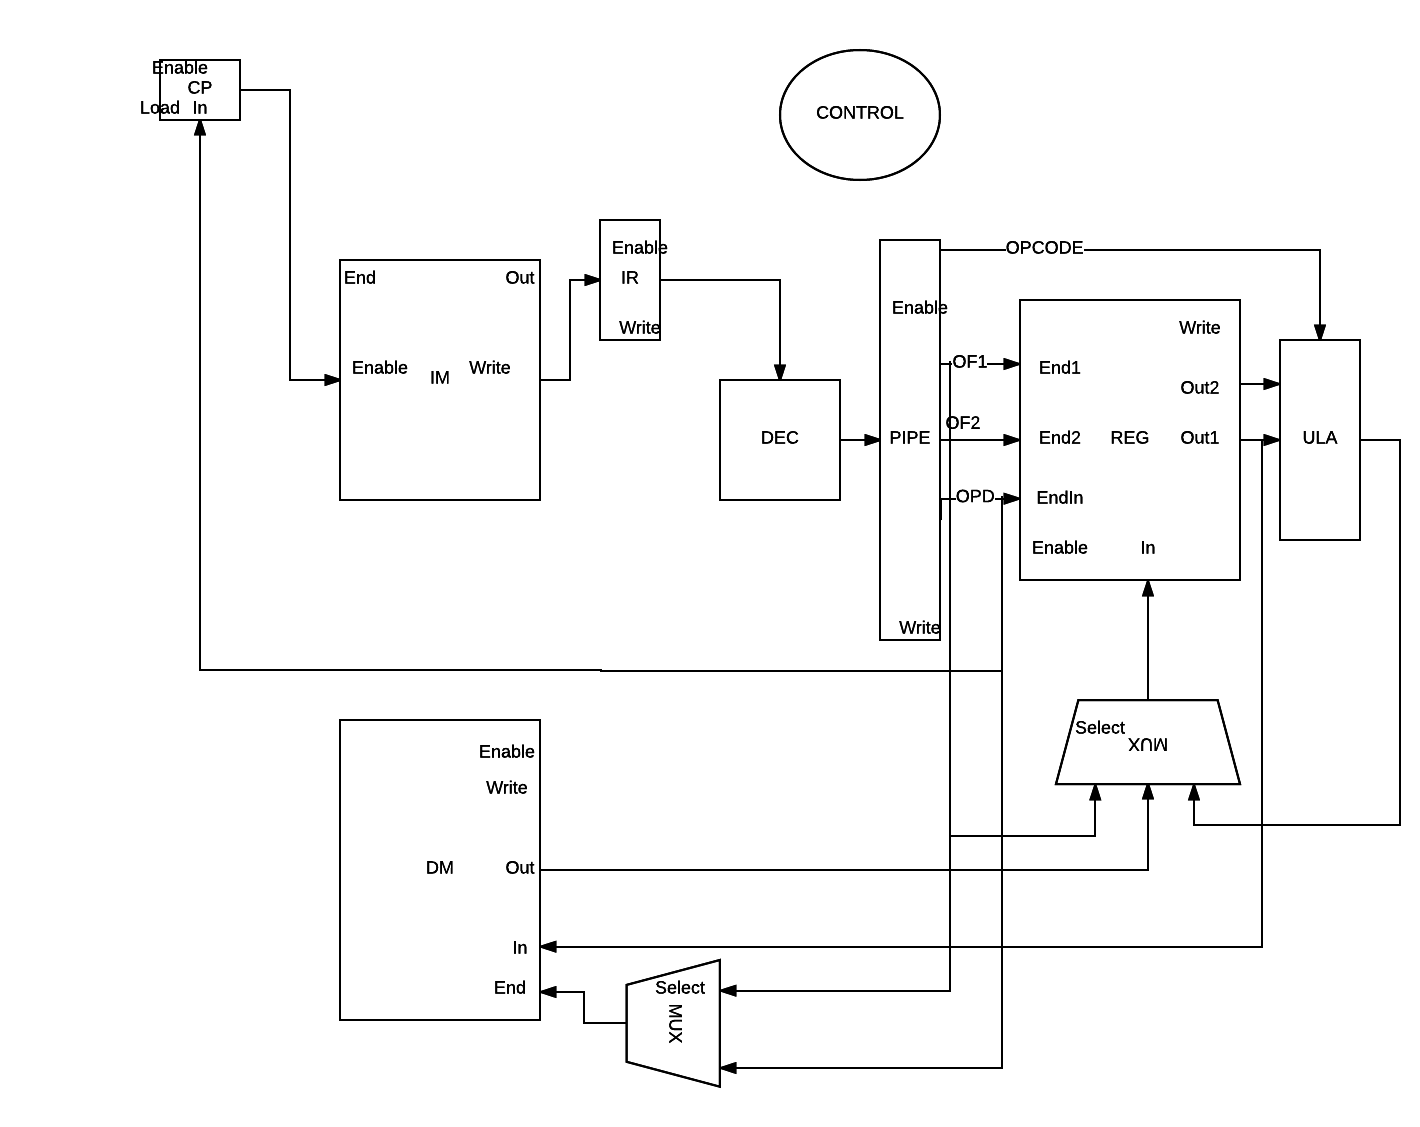
\includegraphics[scale=0.5]{img/procdiag}
	\caption{Diagrama de blocos da parte operativa.}
	\label{fig:op}
\end{figure}


\subsection{Parte de controle}
A parte de controle consiste em um bloco que recebe a palavra de instrução decodificada
e utiliza uma máquina de estados para gerar os sinais de controle adequados
a cada microinstrução. O diagrama de estados está abaixo representado:

\begin{figure}[H]
	\centering
	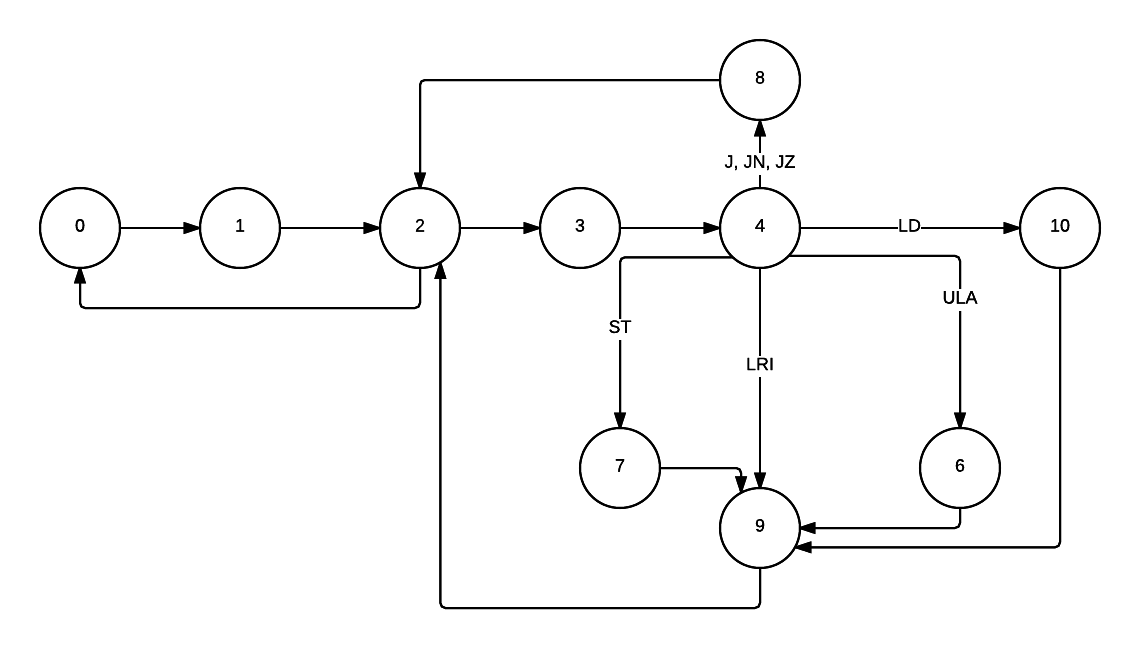
\includegraphics[scale=0.6]{img/statediag}
	\caption{Diagrama de estados da parte de controle.}
	\label{fig:op}
\end{figure}

A tabela abaixo descreve o que ocorre em cada estado:

\begin{table}[H]
	\centering
	\begin{tabular}{l | p{10cm}}
		Estado	& Ações\\
		\hline
		0	& Prepara para escrever a instrução no barramento.\\
		1	& Prepara para escrever a instrução no RI.\\
		2	& Caso o pipeline não seja reiniciado, prepara para escrever no
			  registrador de pipeline. Caso seja, envia para o estado 0.\\
		3	& Desabilita escrita no pipeline, prepara nova instrução para o
			  barramento do RI (pipelining).\\
		4 	& Prepara a execução da instrução de fato e a escrita no RI da 
			  próxima instrução (pipelining).\\
		6	& Desabilita sinais após a execucação da ULA.\\
		7	& Desabilita sinais após a escrita na memória.\\
		8	& Desabilita escrita no CP e envia para o estado 2, para
			  reiniciar o processo.\\
		9	& Desabilita sinais após guardar os resultados no banco de registradores.\\
		10	& Prepara execução da operação de LD.\\
		\hline
	\end{tabular}
\end{table}

\newpage

\section{Implementação}

O processador foi implementado por meio da biblioteca SystemC, versão 2.3.1. Cada
módulo do diagrama de blocos foi implementado separadamente, de forma a manter
uma boa organização do projeto.

Nos arquivos que acompanham este documento, está o \emph{script} {\ttfamily compile.sh} necessário
para se compilar o processador. Para algumas máquinas, talvez seja preciso
editar a linha de compilação, pois são utilizadas variáveis de sistema
que podem ser alteradas dependendo do método de instalação da 
biblioteca\footnote{Seguimos a instalação contida em 
\url{http://chaitulabs.blogspot.com.br/2014/05/systemc-231-installation-in-ubuntu.html}.}.
Note que o arquivo a ser compilado é o {\ttfamily processor\_run.cpp}.

Uma vez compilado, basta executar o arquivo resultante passando como argumento
um arquivo contendo o algoritmo.

\subsection{Testes}
Para testar o funcionamento do processador e do pipeline, os seguintes algoritmos foram utilizados:

\begin{description}
	\item [3x6] Realiza a multiplicação $3 \times 6$ e armazena na memória:

	\begin{lstlisting}
LRI 1 3
LRI 2 6
LRI 3 1
LRI 4 0
LRI 5 0
CMP 9 4 1
JZ 10
ADD 5 5 2
SUB 1 1 3
J 5
ST 1 5
	\end{lstlisting}

	\item [Fib(10)] Computa o décimo elemento da sequência de Fibonacci e o armazena
		na memória:

\begin{lstlisting}
LRI 3 1    
LRI 6 0   
LRI 7 1   
LRI 1 0   
LRI 2 1   
LRI 4 1   
LRI 5 10  
SUB 5 5 7 
CMP 9 5 4 
JN 15	  
ADD 3 1 2 
ADD 1 6 2 
ADD 2 6 3 
ADD 4 7 4 
J 8	
ST 1 3
\end{lstlisting}

	\item [Logic] Realiza todas as operações lógicas possíveis com o processador
		em operandos advindos da memória de dados:

\begin{lstlisting}
LRI 0 2
LRI 1 3
ST 0 0
ST 1 1
LD 2 0
LD 3 1
ADD 4 3 2
SUB 5 4 3
AND 6 1 2
OR 7 1 2
XOR 8 1 2
NOT 9 1
\end{lstlisting}

\end{description}

Além disso, testou-se cada instrução separadamente, em busca do número de ciclos que cada uma leva.
Manteve-se o número de ciclos necessários para se detectar a parada do programa. 
\subsection{Resultados}

Nos testes individuais das instruções, os resultados foram os seguintes:

\begin{table}[H]
\centering
\begin{tabular}{l | r}
Instrução & Ciclos\\
	\hline
    AND & 9\\ 
    OR  & 9\\
    XOR & 9\\
    NOT & 9\\
    CMP & 9\\
    ADD & 9\\
    SUB & 9\\
    LD  & 9\\
    ST  & 9\\
    J   & 11\\
    JN  & 11\\
    JZ  & 11\\
    LRI & 9\\
\end{tabular}
\label{tab:insttest}
\caption{Ciclos para cada instrução.}
\end{table}

Graças ao pipeline, esse número diferiu para as instruções de \emph{jump}, 
pois ele foi limpo, e a instrução de parada precisou ser processada desde o estágio
0.

A ação do pipeline foi também demonstrada por meio do cálculo de ciclos necessários para se executar
cada um dos três programas listados na seção anterior. 
A tabela abaixo apresenta os resultados alcançados:

\begin{table}[H]
	\centering
	\begin{tabular}{c | c | c}

	Algoritmo	& Ciclos sem pipeline	& Ciclos com pipeline\\
	\hline
	3x6		& 149			& 115		     \\
	Fib(10)		& 492			& 374		     \\
	Logic	        & 82			& 58		     \\
	\hline
	\end{tabular}
	\caption{Resultados de execução dos algoritmos de teste.}
	\label{tab:resultados}
\end{table}

Quanto à corretude, todas as operações culminaram nos resultados
esperados.

\newpage

\section{Conclusões}
Ao final do projeto, concebeu-se um processador RISC muito simples,
com instruções lógico-aritméticas, de controle e de movimentação
de dados. O pipeline também foi orientado à simplicidade, contendo
apenas um estágio, localizado entre a busca da instrução e a execução, 
e sempre sendo esvaziado quando diante de uma instrução de \emph{jump}.
Ainda assim, os resultados mostram uma redução notável no número de ciclos.
Certamente, o grupo tem consciência de que a implementação de mais estágios
aumentaria consideravelmente a eficiência do processador.

Em termos de aprendizado, este trabalho proporcionou um melhor entendimento
quanto ao que foi ensinado durante a disciplina. Criar um processador 
desde as decisões de projeto foi importante para que se compreendesse
o valor de um bom planejamento para guiar o desenvolvimento da descrição
de \emph{hardware} e obter os resultados desejados nas simulações. 
Além disso, a opção pelo SystemC permitiu que fossem
incorporadas novas técnicas, somadas às adquiridas com VHDL na disciplina
de Circuitos Lógicos (2016.1).
\end{document}
